\section{Evaluation}
\label{sec:evaluation}

\subsection{Storage Capacity}
\label{subsec:capacity}
\begin{figure}[t]
	\centering
	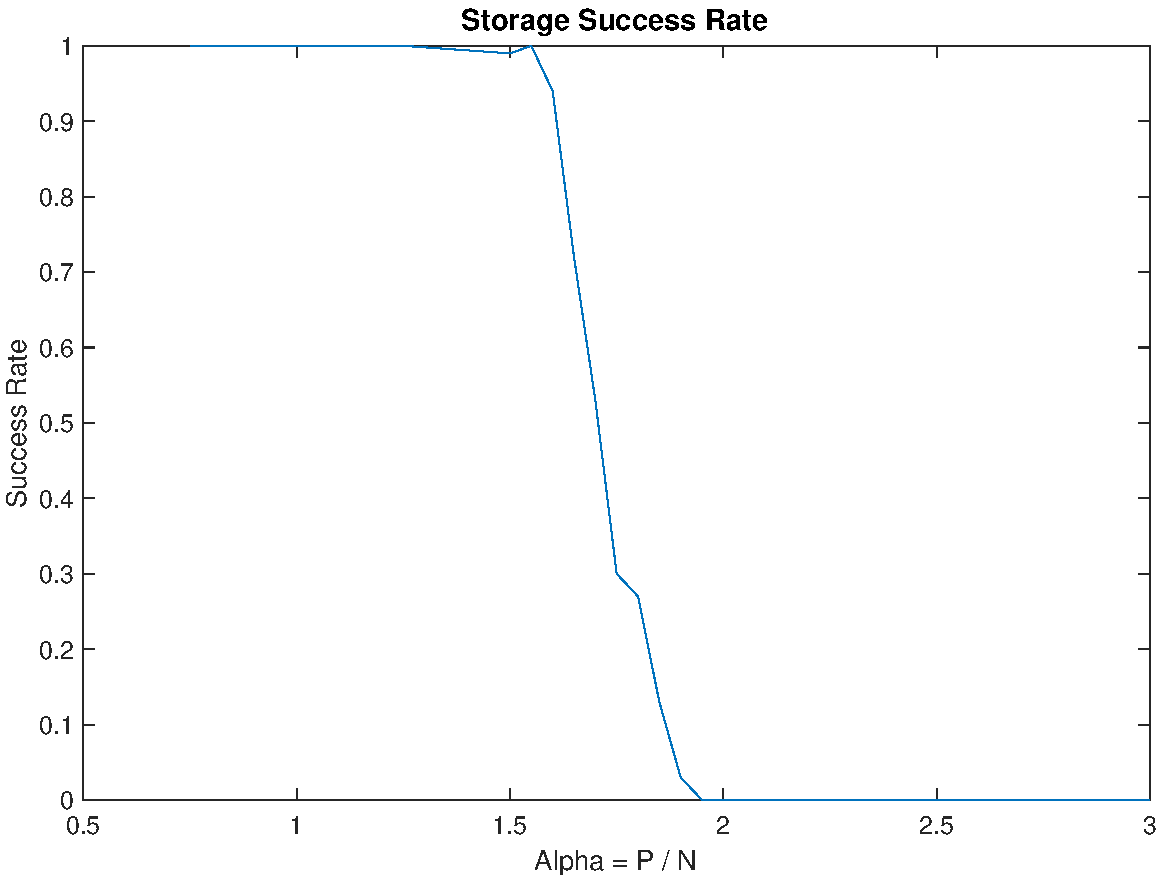
\includegraphics[width=\columnwidth]{figures/base}
    \caption{Storage success rate of a Rosenblatt perceptron as a function of $\alpha = P / N$. The experiments use $N = 500$, $n_{max} = 200$ and $n_D = 100$.}
	\label{fig:base}
\end{figure}

\cref{fig:base} shows the results of the base experiment using $N = 500$, $n_{max} = 200$ and $n_D = 100$.
The x-axis represent different values of $\alpha = P / N$, while the y-axis the success rate $Q_{l.s.}$.
As expected, the function looks like a step function from $1$ to $0$.
For $\alpha \approx 1.7$, the success rate $Q_{l.s.}$ drops from $1$ to $0$ very quickly. 

The value of $\alpha$ for which the function drops is called storage capacity of the perceptron.
For $N \to \infty$ (very large number of examples) and $n_{max} \to \infty$ (no limit on the maximum number of training epochs), the theoretical storage capacity of the Rosenblatt perceptron is $\alpha = 2$.

\subsection{Number of Epochs}
\label{subsec:epochs}
\begin{figure}[t]
	\centering
	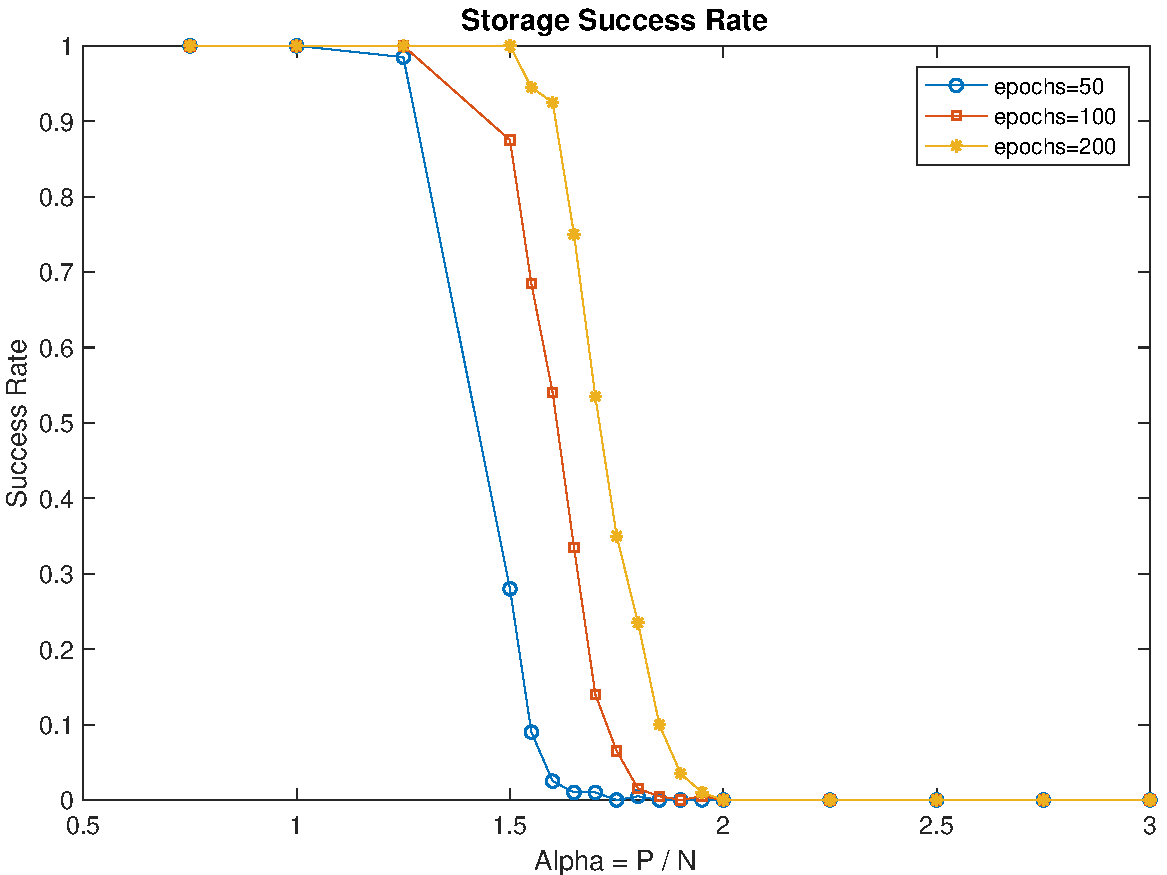
\includegraphics[width=\columnwidth]{figures/multiple_epochs}
    \caption{Storage success rate of a Rosenblatt perceptron as a function of $\alpha = P / N$ for different values of $n_{max}$.}
	\label{fig:multiple_epochs}
\end{figure}

The difference between the theoretical value and the experimental one are mainly due to the limited number of training epochs.
\cref{fig:multiple_epochs} gives an experimental proof of this statement:
for a very small number of epochs (eg. $n_{max} = 10$), the step is close to $\alpha = 1$, while for higher values of epochs the step moves closer and closer to the theoretical value $\alpha = 2$.

\subsection{Number of Dimensions}
\label{subsec:dimensions}
\begin{figure}[t]
	\centering
	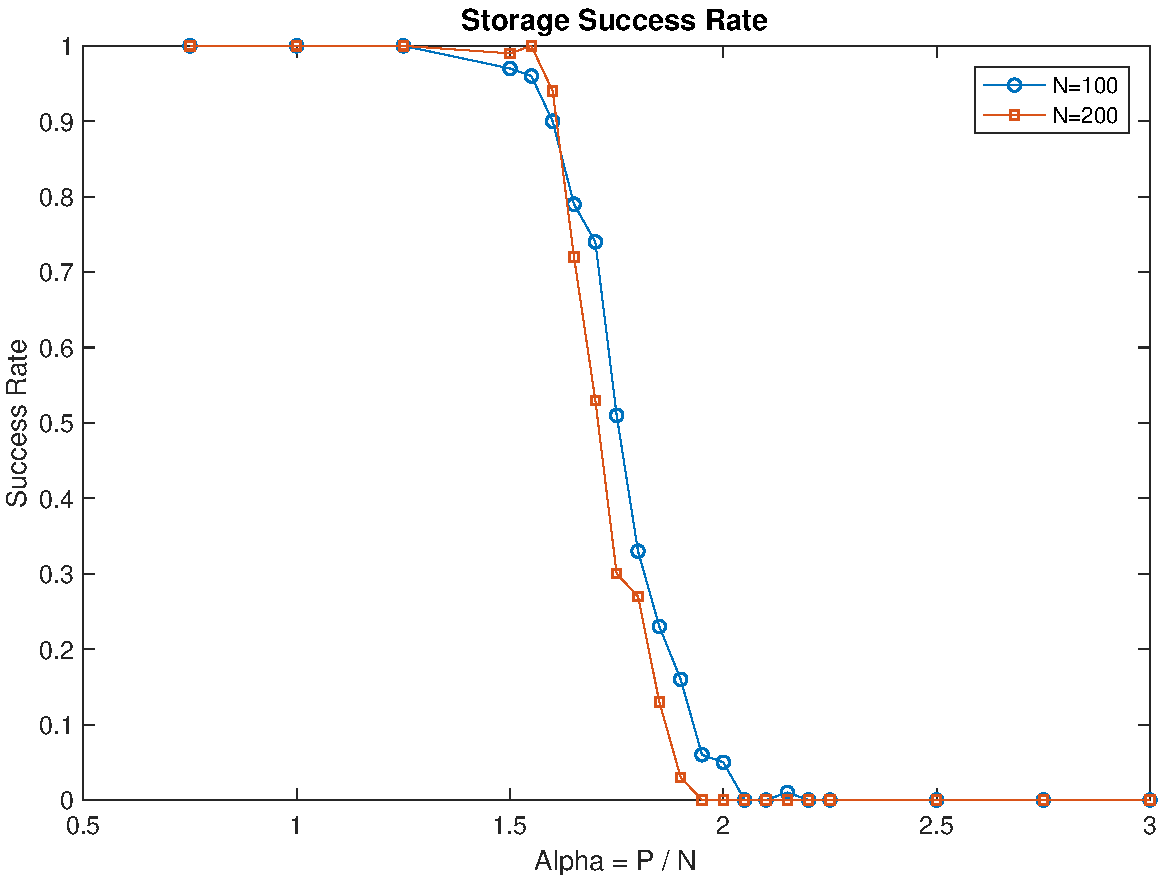
\includegraphics[width=\columnwidth]{figures/multiple_n}
    \caption{Storage success rate of a Rosenblatt perceptron as a function of $\alpha = P / N$ for different values of $N$.}
	\label{fig:multiple_n}
\end{figure}

The theoretical results are valid for $N \to \infty$.
However, real datasets have a limited number of features.
\cref{fig:multiple_n} shows the behaviour of the perceptron for different values of $N$.
For high values of $N$, the shape of the success rate $Q_{l.s.}$ as a function of $\alpha$ is similar to a step function.
For small values of $N$, the function looks like a smoothed step function:
the smaller $N$ is, the higher is the smoothing.

\subsection{Value of $c$}
\label{subsec:c}
TODO... sam

\subsection{Inhomogeneous Hyperplanes}
\label{subsec:homogeneous}
\begin{figure}[t]
	\centering
	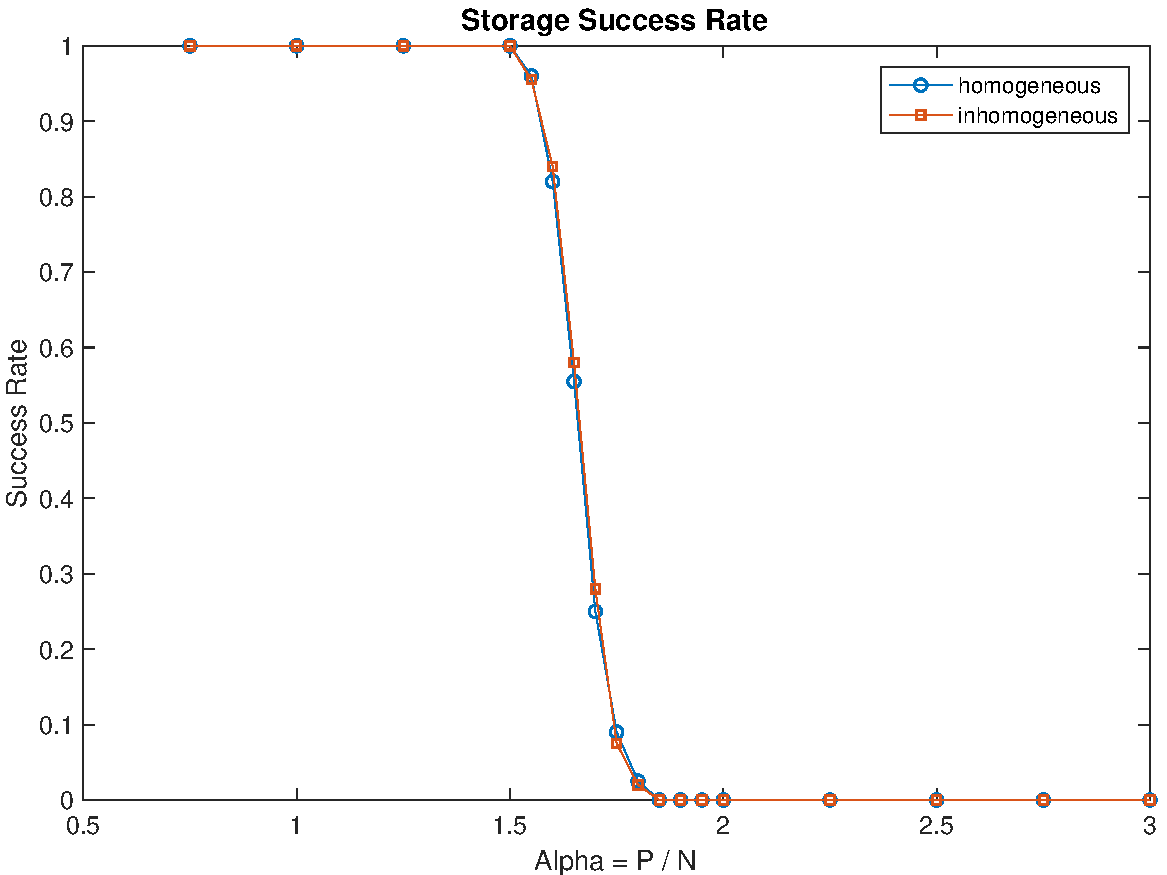
\includegraphics[width=\columnwidth]{figures/homogeneous}
    \caption{Storage success rate of a Rosenblatt perceptron and its inhomogeneous version as a function of $\alpha = P / N$.}
	\label{fig:homogeneous}
\end{figure}

Rosenblatt perceptrons only learns separation hyperplanes that goes through the origin (homogeneous).
In general, a solution to the classification problem may be a hyperplane that does not go through the origin (inhomogeneous).
It is possible to generalize the Rosenblatt perceptron to learn also inhomogeneous separation hyperplanes by adding an artificial dimension to the dataset and forcing it to a non-zero constant (e.g. $1$):
it is easy to prove that each dataset inhomogeneously linearly separable in $R^N$ is homogeneously linearly separable in $R^{N+1}$.

We run an experiment to verify the behaviour of $Q_{l.s.}$ by allowing inhomogeneous hyperplanes:
we trained both a normal and modified perceptron on $200$ different datasets using $N = 500$, $n_max = 200$. 
\cref{fig:homogeneous} shows the results of the experiment.
As expected, the success rate $Q_{l.s.}$ of the inhomogeneous perceptron is slightly higher than homogeneous one.
However, the difference is not significant.

Since finding a homogeneously solution in $R^{N+1}$ is equivalent to find an inhomogeneously solution ... TODO!

\begin{figure}[t]
	\centering
	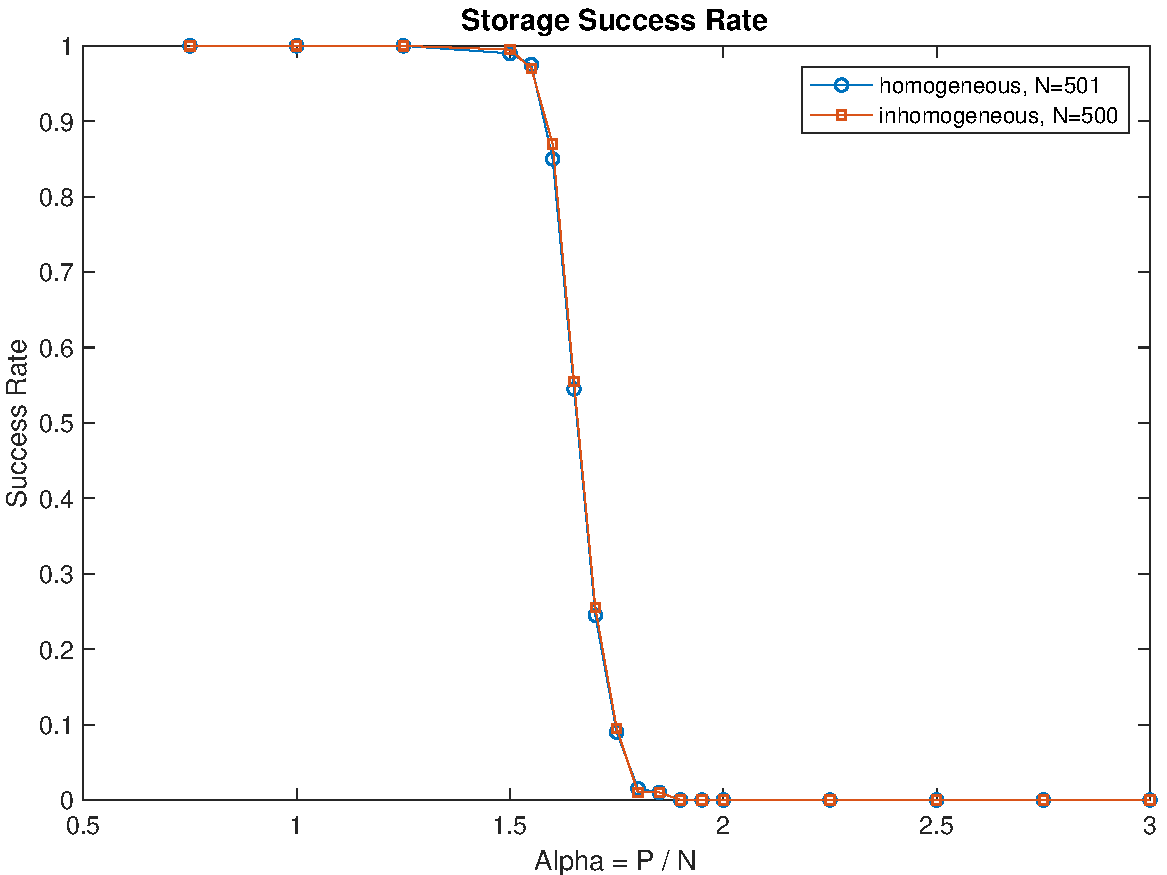
\includegraphics[width=\columnwidth]{figures/homogeneous_n_n1}
    \caption{TODO.}
	\label{fig:homogeneous_n_n1}
\end{figure}

\subsection{TODO}
\begin{itemize}
    \item With a limited number of epochs and repetitions the algorithm doesn't have enough time to approach its theoretical values
    \item C seems to be related to the learning rate
    \item say how we choose values for alpha...
    \item Description of plots!
\end{itemize}
